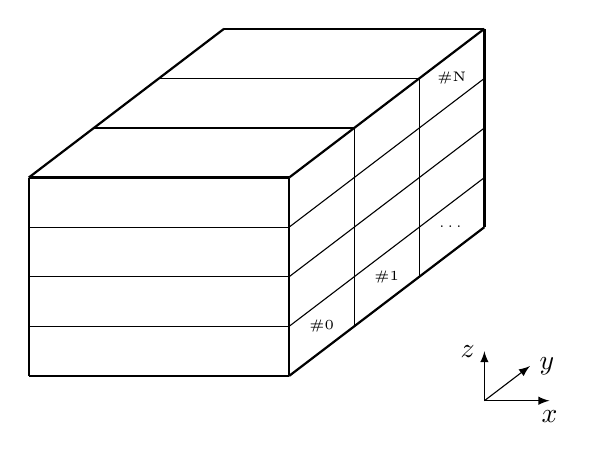
\begin{tikzpicture}[scale=1.4]
\begin{scope}[x={0 250},y={0 200}]
%        %% next four lines will help you to locate the point needed by forming a grid. comment these four lines in the final picture.↓
%        \draw[help lines,xstep=.1,ystep=.1] (0,0) grid (1,1);
%        \draw[help lines,xstep=.05,ystep=.05] (0,0) grid (1,1);
%        \foreach \x in {0,1,...,9} { \node [anchor=north] at (\x/10,0) {0.\x}; }
%        \foreach \y in {0,1,...,9} { \node [anchor=east] at (0,\y/10) {0.\y};}
%        %% upto here↑

% domain
\draw[thick] (0.1,0.1) -- (0.5,0.1);
\draw[thick] (0.1,0.1) -- (0.1,0.5);
\draw[thick] (0.1,0.5) -- (0.5,0.5);
\draw[thick] (0.5,0.1) -- (0.5,0.5);
\draw[thick] (0.5,0.1) -- (0.8,0.4);
\draw[thick] (0.5,0.5) -- (0.8,0.8);
\draw[thick] (0.8,0.4) -- (0.8,0.8);
\draw[thick] (0.1,0.5) -- (0.4,0.8);
\draw[thick] (0.4,0.8) -- (0.8,0.8);

% axis
\draw[-latex] (0.8,0.05) -- (0.9,0.05)node[anchor=north]{$x$};
\draw[-latex] (0.8,0.05) -- (0.8,0.15)node[anchor=east]{$z$};
\draw[-latex] (0.8,0.05) -- (0.87,0.12)node[anchor=west]{$y$};

% decomposition
\draw (0.1,0.2) -- (0.5,0.2);
\draw (0.1,0.3) -- (0.5,0.3);
\draw (0.1,0.4) -- (0.5,0.4);
\draw (0.8,0.5) -- (0.5,0.2);
\draw (0.8,0.6) -- (0.5,0.3);
\draw (0.8,0.7) -- (0.5,0.4);
\draw (0.6,0.2) -- (0.6,0.6);
\draw (0.7,0.3) -- (0.7,0.7);
\draw (0.2,0.6) -- (0.6,0.6);
\draw(0.3,0.7) -- (0.7,0.7);

% ranks
\draw (0.55,0.2)node[rotate=0]{\tiny{\#0}};
\draw (0.65,0.3)node[rotate=0]{\tiny{\#1}};
\draw (0.75,0.4)node[rotate=0]{\tiny{\dots}};
\draw (0.75,0.7)node[rotate=0]{\tiny{\#N}};

\end{scope}
\end{tikzpicture}
